Una imagen puede ser interpretada como una función bidimensional $f\left( x, y\right)$, donde tanto $x$ como $y$ representan en un plano el espacio visualizado, mientras que la misma función $f\left( x, y\right)$ es la intensidad de la imagen bajo un punto dado. Cuando $x$, $y$ y $f\left( x, y\right)$ son valores cuantizados y discretizados, la imagen se transforma en una imagen digital.

%f(x, y) como un campo vectorial cuya salida es un vector de intensidad y frecuencia
	 	
El procesamiento de dichas se define como el conjunto de técnicas aplicadas a estas imágenes, con el objetivo extraer información de ellas. Estas actividades cubren un campo que abarca un sin fin de aplicaciones, ya que se vale de maquinas capaces de detectar la totalidad del espectro electromagnético. Esto significa que se pueden obtener imágenes generadas por fuentes que captan información la cual para los humanos no se asocian con imágenes propiamente dichas, como lo son las ondas de radio, entre tantas otras.
	
Es posible considerar tres tipos de procesos computarizados en el procesamiento de imágenes, basándose en el nivel de tratamiento que se aplique, siendo así clasificados en bajo, medio y alto nivel. Los primeros incluyen actividades tales como reducción de ruido y aumento de contraste, tareas caracterizadas por el hecho de que tanto la entrada como la salida son imágenes. Las actividades de medio nivel de procesamiento incluyen trabajos de segmentación, es decir, identificar regiones u objetos dentro de las imágenes, descripción y clasificación de dichos elementos. Es así que esta categoría es destacada por sus salidas, ya que suelen ser información extraída de las imágenes a la entrada. Por último, los procesos de alto nivel se caracterizan por no solo reconocer objetos y analizarlos, sino también por darles un tratado normalmente asociado con la visión, tales así como ``darles sentido'' \cite{ref:intro1}.
	
Dada una señal continua a la entrada del sistema, una imagen sufre de dos procesos claves: \textbf{cuantización} y \textbf{discretización}. Si bien ambos refieren a tomar variables continuas y almacenarlas en memoria como variables discretas, se realiza esta diferenciación entre ambas ya que la primera hace referencia a la amplitud de la señal mientras que la segunda a coordenadas, que para el caso del estudio de imágenes, se refiere a pixeles. Estos son el mínimo elemento que compone una imagen digital y se pueden pensar como un cuadrado de color uniforme.
	
Ejemplificando lo anterior, se toma una entrada al sistema, como puede ser la presentada en la Figura (\ref{fig:disc1}), la cual, como ya se ha mencionado, es continua en $x$, $y$ y $f(x,y)$.
\begin{figure}[H]
\centering
	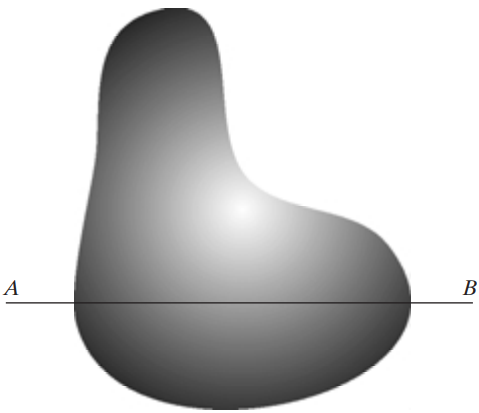
\includegraphics[width=0.3\textwidth]{Imagenes/Digitalizacion_1.png}
	\caption{Entrada continua al sistema.}
	\label{fig:disc1}
\end{figure}

Por lo tanto, se deben tomar coordenadas finitas, por ejemplo, aquellas que se encuentran sobre la recta AB, y asignarle a cada una un valor dado de amplitud. En la Figura~(\ref{fig:disc2}) se observa como una recta continua paralela al eje $x$ (horizontal), la cual posee ciertas variaciones aleatorias dadas por el ruido existente, es dividida en una cierta cantidad de posiciones equiespaciadas (discretización), marcadas con cuadrados blancos sobre la curva, asignándoles un nivel específico en la escala de grises (cuantización), marcado con una linea negra por la izquierda de dicha escala.
\begin{figure}[H]
\centering
	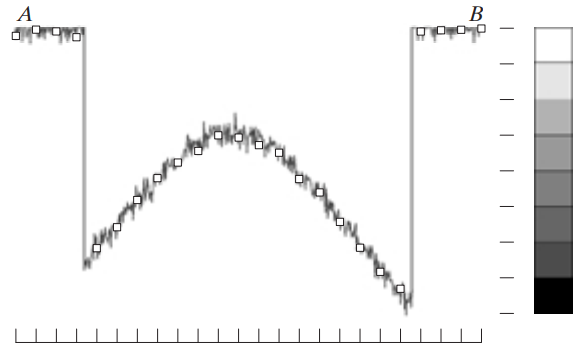
\includegraphics[width=0.4\textwidth]{Imagenes/Digitalizacion_2.png}
	\caption{Amplitud de la escala de grises en la recta AB y muestreo de valores.}
	\label{fig:disc2}
\end{figure}

Realizando el mismo proceso para todos los niveles de discretización en el eje $y$ (vertical), se obtiene finalmente una imagen digitalizada, la cual se la compara a continuación con la original \cite{ref:digit1}.
\begin{figure}[H]
\centering
	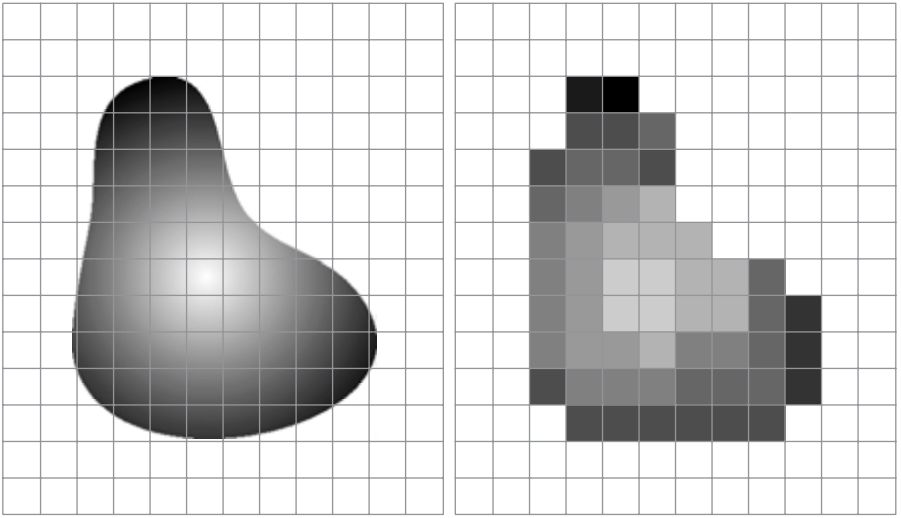
\includegraphics[width=0.5\textwidth]{Imagenes/Digitalizacion_3.png}
	\caption{Imagen original comparada con la imagen digitalizada a procesar.}
	\label{fig:disc3}
\end{figure}

Este trabajo se centra en procesos de medio nivel. Dicha definición es muy amplia, por lo cual es necesario acotar este camino. Es por ello que se decidió centrarse en el seguimiento de objetos en imágenes en movimiento. Se buscó que, dada ciertas condiciones iniciales conocidas (brindadas por el usuario) en una imagen en movimiento en tiempo real, tomar un conjunto de datos de $x$, $y$ y $f(x,y)$ para así seleccionar un elemento y seguir su trayectoria a través del tiempo. Como hipótesis plantearemos:
\begin{itemize}
\item El objeto no cambiará rápidamente de color ni su iluminación o exposición-
\end{itemize}
Para esto, se utilizaron los algoritmos de Shi-Tomasi, Optical Flow de Lucas-Kanade asimismo como filtros de correlación, de Kalman y de probabilidad de distribución de color.